\documentclass[a1paper, portrait, margin=0mm, innermargin=15mm,blockverticalspace=15mm, colspace=15mm, subcolspace=8mm]{tikzposter} 
	\usepackage{graphicx}
	\usepackage{capt-of}
	\usepackage{pgfplots}
	\usepackage{natbib}
	\usepackage{hyperref}

    \title{Attacking Microcontrollers} 
 %   \institute{Schoold of Electronics and Computer Science, University of Southampton}
    \author{Author: Dionisio Perez-Mavrogenis (dpm3g10)\\
			Supervisor: Klaus-Peter Zauner (kpz)}
    \usetheme{Board} %Board is also cool

\definetitlestyle{sampletitle}{
	width=500mm, roundedcorners=20, linewidth=2pt, innersep=2pt,
	titletotopverticalspace=7mm, titletoblockverticalspace=10mm
	}{
	\begin{scope}[line width=\titlelinewidth, rounded corners=\titleroundedcorners]
		\draw[color=blocktitlebgcolor, fill=titlebgcolor]
		(\titleposleft,\titleposbottom) rectangle (\titleposright,\titlepostop);
		\end{scope}
	}
   \usetitlestyle{sampletitle}
\definebackgroundstyle{die_image}{
\includegraphics[height=\paperheight, width=\paperwidth]{opt.jpg}
}
\usebackgroundstyle{Rays}    
    
\begin{document}
\bibliographystyle{plain}
\maketitle     
    \begin{columns} % See Section 4.4
        \column{0.5} % See Section 4.4
            \block{Microcontroller Introduction}{
                Microcontrollers can be found anywhere, from your cars stereo to missile launch panels and are usually cheap (around \pounds 2) and packed with information! They often come with crypto-engines (AES, DES and RSA are common) and hold all sorts of information like private crypto-keys for authentication or proprietary algorithm implementations in the firmware or hardware, interesting all sorts of people into the contents of a microcontroller.
} % end introduction block
            \block{Packaging and De-packaging}{
				Typically microcontrollers are too small and fragile to use as fabricated and so they are packaged. Packaging material ranges depending on the microcontroller and its intended use,  but is usually hard epoxy resin \citep{sergei:thesis} \citep{hwre}. The packaging tries to protect the microcontroller from its external environment (humidity, radiation, temperature, crashes etc.) and also from prying eyes. Military-grade chips come with a lot of additional circuitry on the packaging whose responsibility is to detect tampering and respond in a suitable manner (even self destruction!) \citep{hwre}.\\
               De-packaging is not always required and the methods depend on the packaging used and protective mechanisms in place, but on epoxy-packaged chips one can etch the epoxy away by using HNO$_3$ or H$_2$SO$_4$ and then cleaning the chip in an ultrasonic bath \citep{sergei:thesis} \citep{hwre}. For other packaging types, e.g. metal, ceramic or plastic, one can use similar techniques and tools, e.g. drills or a blowtorch \citep{hwre}.De-packaging is usually easier than expected and removing simple epoxy resin can be done with readily available chemicals \citep{hwre}. Fig.~\ref{328c} and Fig.~\ref{328o} show a microcontroller in its factory resin packaging and the exposed die after chemical decapsulation\citep{siliconpr0n_328}.

		\begin{minipage}{0.5\linewidth}
			\begin{tikzfigure}[{\tiny ATmega328 with epoxy resin packaging.}]
				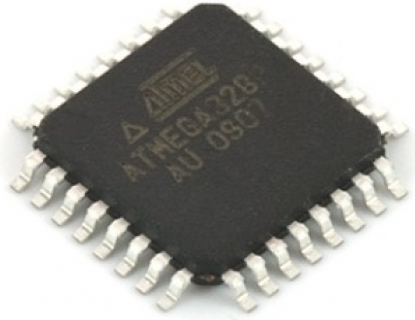
\includegraphics[width=0.7\textwidth]{atmega328.jpg}
				\label{328c}
			\end{tikzfigure}
		\end{minipage}% <--- the percent character will "comment out" the new line    
		\begin{minipage}{0.5\linewidth}
			\begin{tikzfigure}[{\tiny The exposed die of an ATmega328.}]
				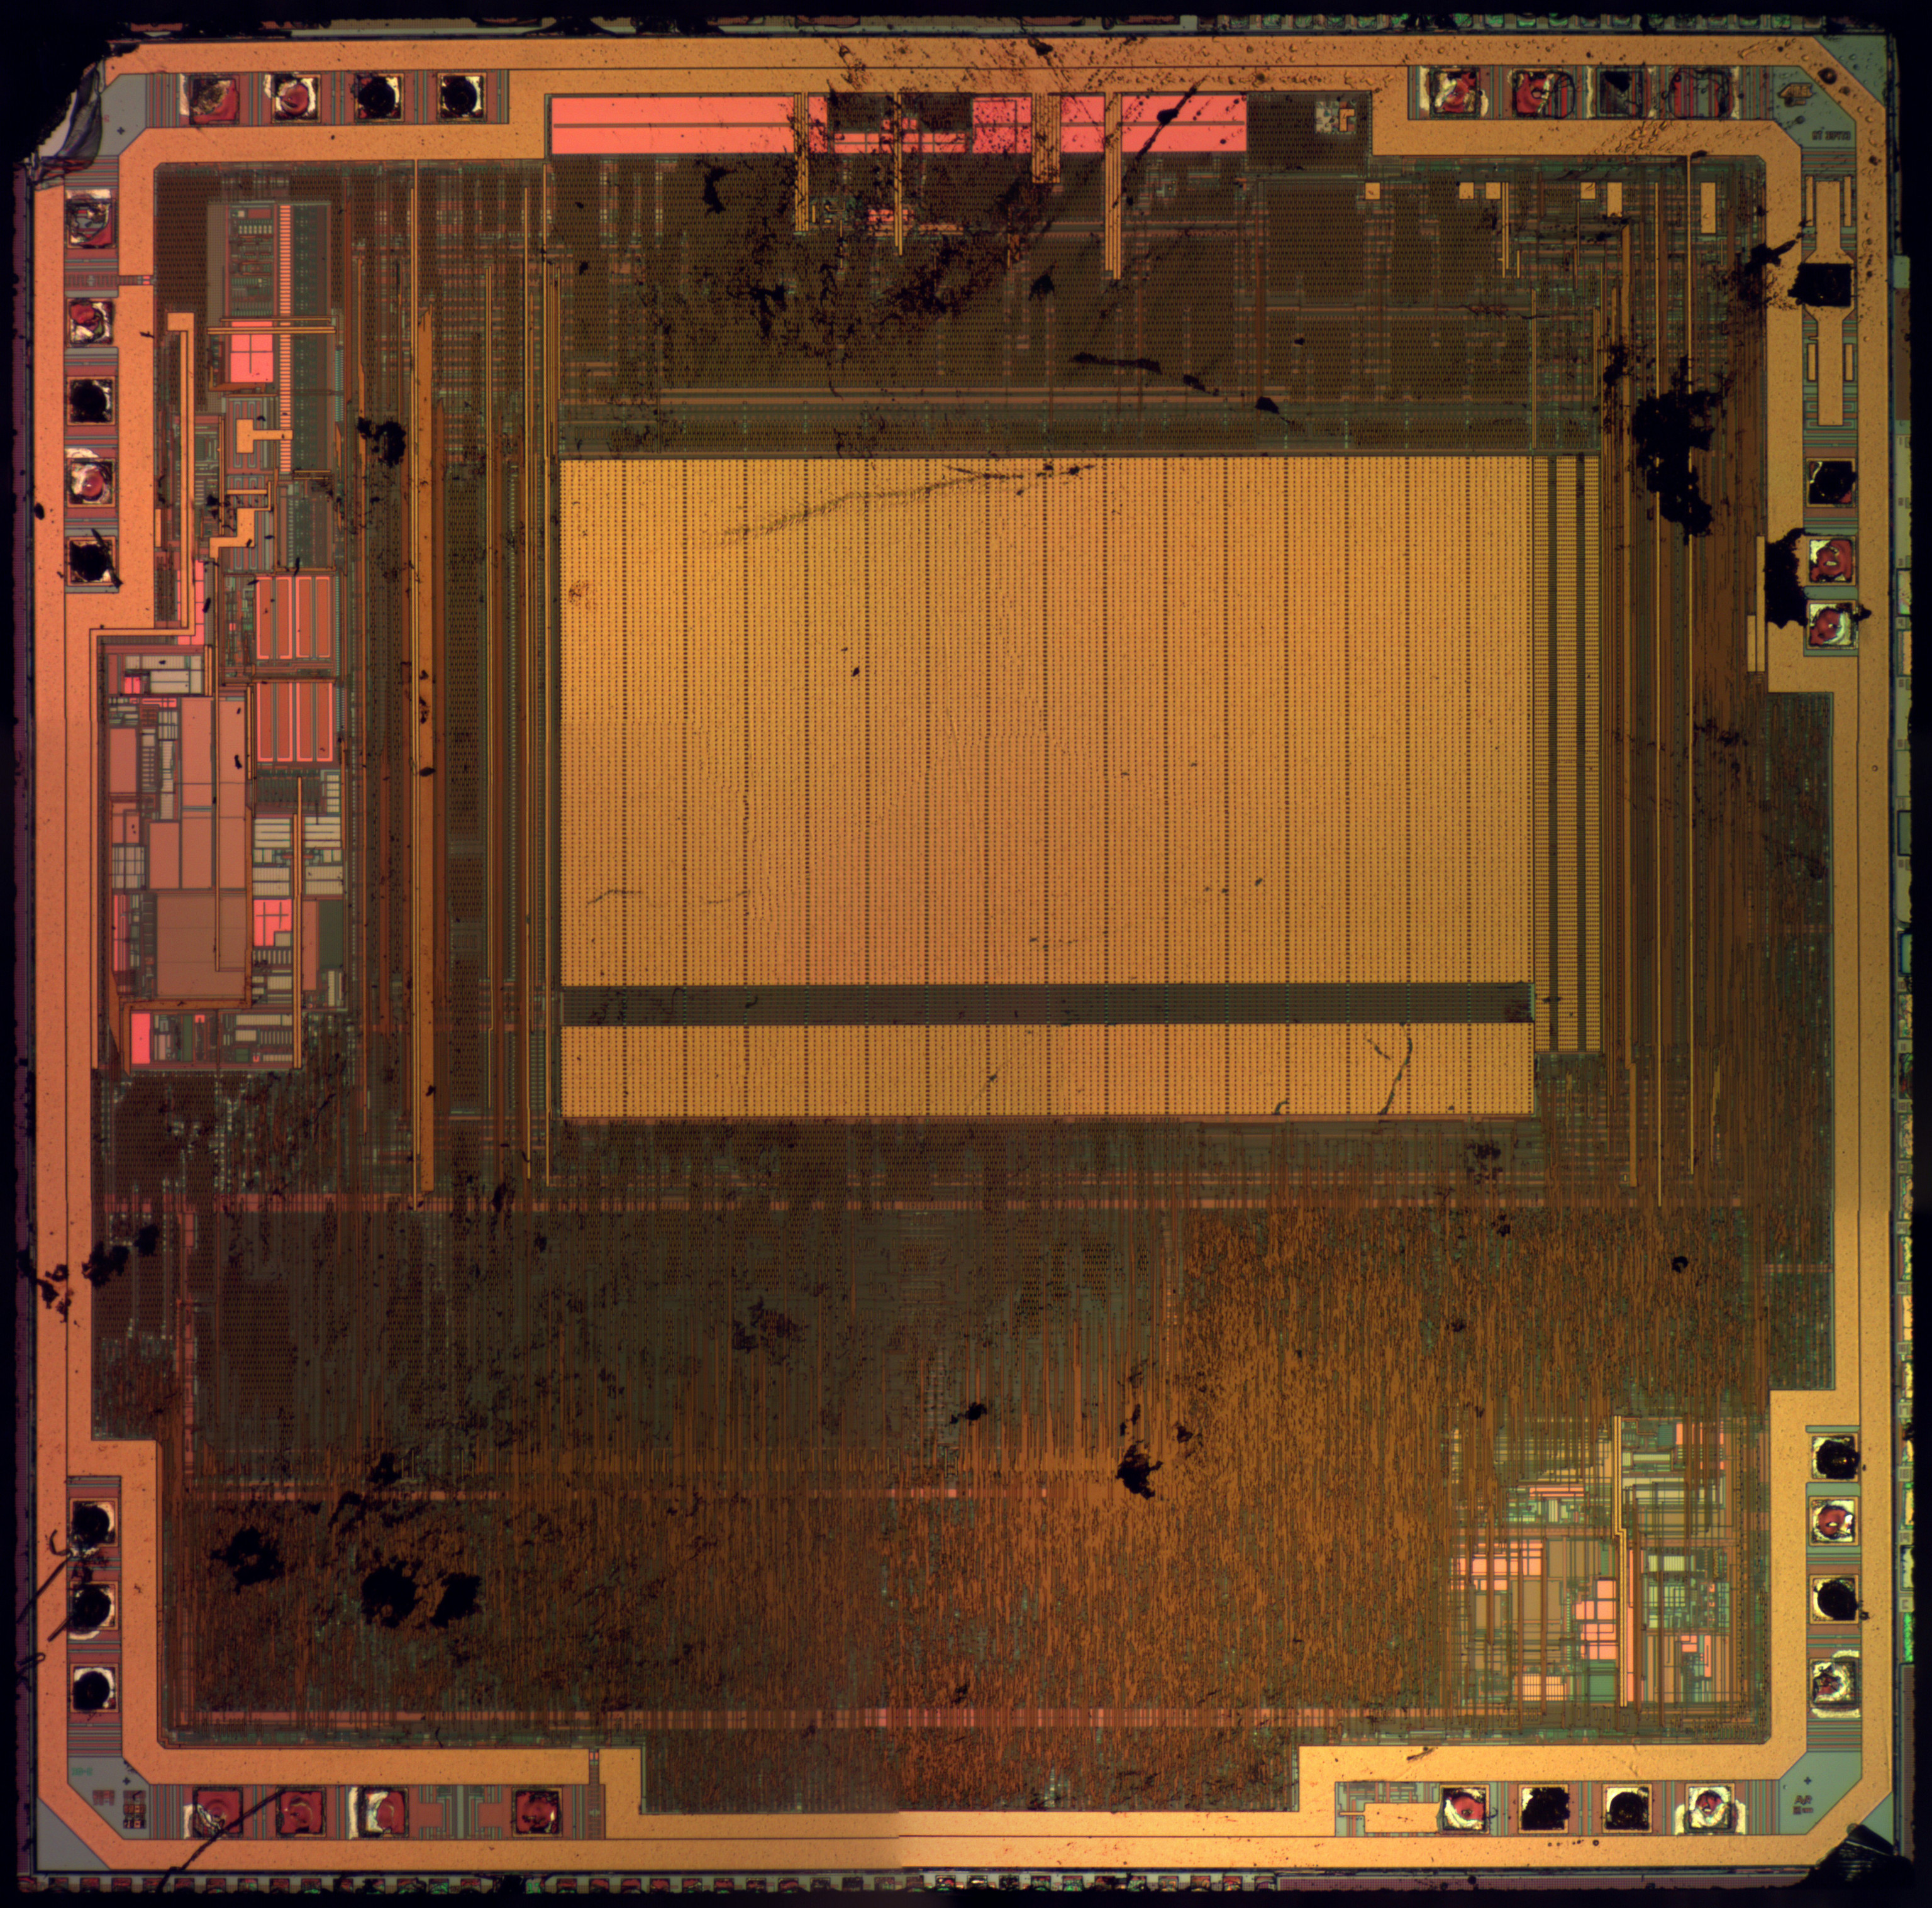
\includegraphics[width=0.7\textwidth]{atmega328_open.jpg}
				\label{328o}
			\end{tikzfigure}
		\end{minipage}
}% end packaging block

%            \note[rotate=15, width=15cm, targetoffsetx=5cm,targetoffsety=-5cm]{tampering detection means detecting abnormalities in voltage, clock frequency, radiation, tilting etc.}
\block[roundedcorners=65]{}{{\tiny \bibliography{poster}}}
        \column{0.5}
        	\block{Attack Types}{
				\textbf{Non-invasive} attacks are cheap and easy to perform and require no decapsulation. Popular methods include are power analysis and fault injection, where faults may be injected by exposing the chip to environmental conditions that it was not meant to work in. \textbf{Non-Invasive} and \textbf{Semi-invasive} attacks are more technical, expensive and lengthier to perform as they require decapsulation and specialized machinery, but yield more information about a die. Attacks under these categories include micro-probing the device, inducing faults using lasers and physical modification of the chip using FIBs \citep{hwre} \citep{sergei:thesis}. 
				
	\begin{minipage}{0.5\linewidth}
			\begin{tikzfigure}[{\tiny DPA trace for DES (source:\protect\citep{kocher:DPA}).}]
				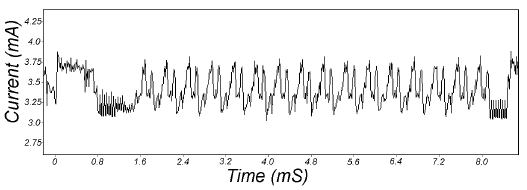
\includegraphics[width=\textwidth]{power_des.png}
				\label{des}
			\end{tikzfigure}
		\end{minipage}% <--- the percent character will "comment out" the new line    
		\begin{minipage}{0.5\linewidth}
			\begin{tikzfigure}[{\tiny Chip modification using FIB (source:\protect\citep{fib_mod}).}]
				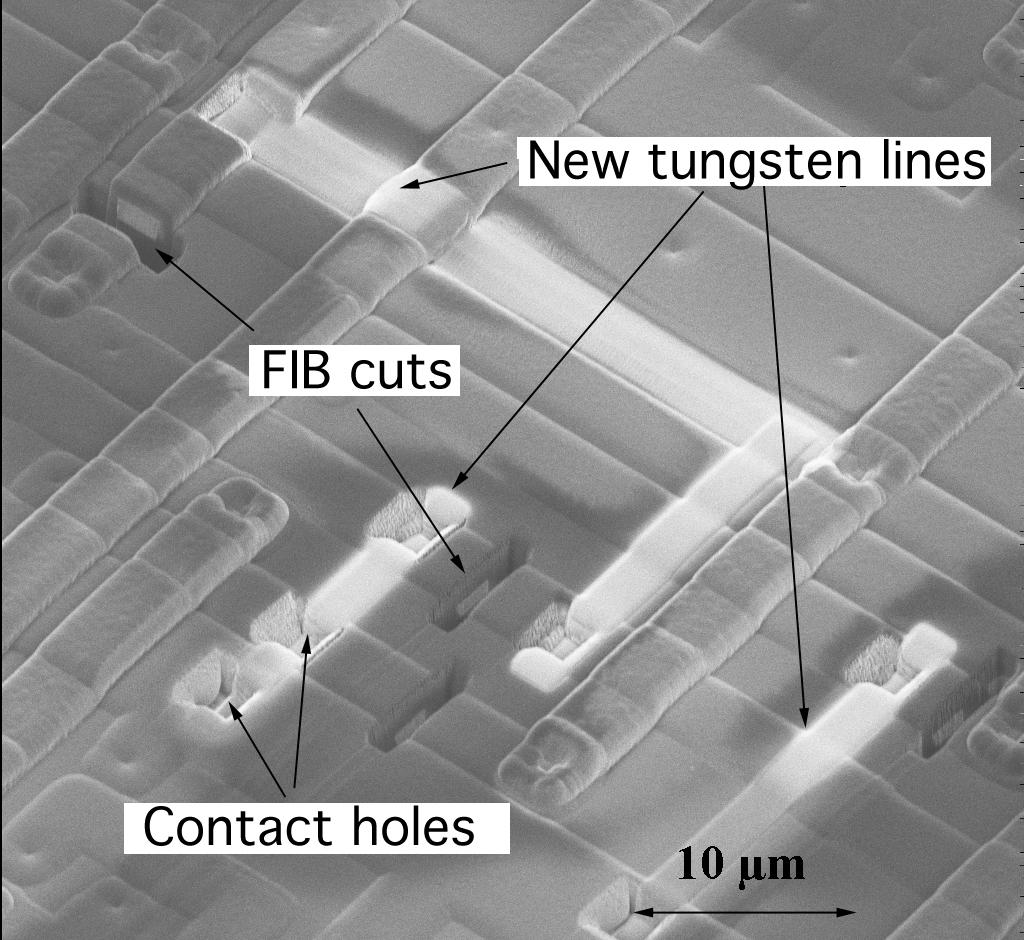
\includegraphics[width=0.7\textwidth]{fib.jpg}
				\label{fib}
			\end{tikzfigure}
		\end{minipage}			
}% end attack types block

            \block{Sample Attack}{
                A simple clock glitch attack could be performed against an ATmega644, in order to make it dump its memory. Since we know how many cycles each instruction takes we would use an FPGA to deliver both the clock signal and the glitch itself, delivering it on the appropriate cycle after a \emph{trigger} event \citep{glitches_paper}\citep{pareja:glitch}.
                
                Suppose we are targeting the loop in the firmware, shown in Fig.~\ref{loop}, outputting to a pin via \texttt{OUT}. We can count the cycles between successive outputs and use the \texttt{OUT} as our trigger, glitching the desired number of cycles after that. We know that targeting single-cycle instructions has the impact of \texttt{NOP}-ing whatever instruction follows without affecting \texttt{PC} incrementation \citep{glitches_paper}, and hence we could keep glitching on \texttt{OUT}'s cycle in order to skip the \texttt{INC R17} operation and thus never make the loop condition false in order to dump as much memory as possible, i.e. view the firmware bytecode.
            
		\begin{minipage}{0.35\linewidth}
			\begin{tikzfigure}[{\tiny Sample glitch generation (source: \protect\citep{glitches_paper}).}]
				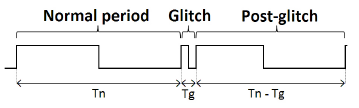
\includegraphics[width=\textwidth]{clock_glitch.png}
				\label{glitch}
			\end{tikzfigure}
		\end{minipage}%       
        \begin{minipage}{0.65\linewidth}
			\begin{tikzfigure}[{\tiny Loop assembly \texttt{while(i<n)\{\}}}.]
				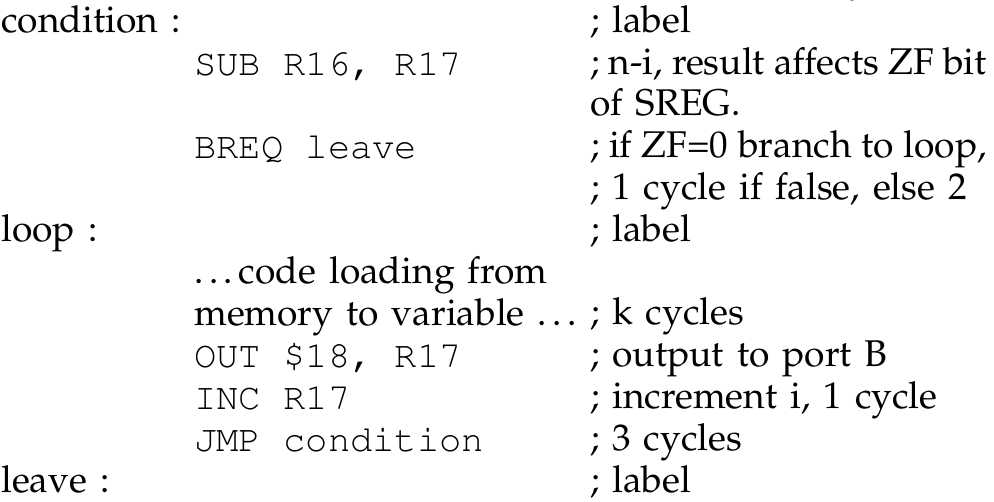
\includegraphics[width=\textwidth]{loop.png}
				\label{loop}
			\end{tikzfigure}
		\end{minipage}    
            
            
} % end sample attack block
    \end{columns}
\end{document}